\chapter{Evaluatie van de voorgestelde voorstellingsmethodes voor klassediagrammen en sequentiediagrammen}\label{sec:evaluatie}
We hebben software ontworpen die een interne voorstelling heeft voor de informatie bevat in een klassediagram en een stel bijhorende sequentiediagrammen. De software kan die interne voorstelling vertalen naar een FO($\cdot$)-theorie opgesteld volgens de regels bekomen in hoofdstukken \ref{sec:consistentie} en \ref{sec:gedrag}. Een XML-vertaler vertaalt een voorstelling van klassediagrammen en sequentiediagrammen in XML naar de interne voorstelling, maar door tijdgebrek is deze vertaler niet doorheen heel het implementatieproces onderhouden geweest.

In dit hoofdstuk ontwerpen we klassediagrammen en sequentiediagrammen waarmee we de spellen Nim en Reversi modelleren. We vertalen die diagrammen dan manueel naar onze interne voorstelling en laten FO($\cdot$)-theorie\"en genereren: een theorie voor Nim en een theorie voor Reversi. We beoordelen de volgende criteria:

\begin{enumerate}
	\item Hoe gemakkelijk is het om tot een ontwerp te komen en hoe omvangrijk is de uitvoertheorie?\label{crit:design}
	\item Kunnen we het spel spelen met de uitvoertheorie?\label{crit:simulation}
	\item Kunnen we verifi\"eren of de uitvoer van bepaalde diagrammen correct is?\label{crit:output}
	\item Kunnen we verifi\"eren of het systeem \textbf{als geheel} beantwoordt aan bepaalde gewenste eigenschappen?\label{crit:properties}
\end{enumerate}

Bij criterium \ref{crit:simulation} beoordelen we de performantie van het spelproces in termen van rekentijd en geheugengebruik. Bij criteria \ref{crit:output} en \ref{crit:properties} doen we dat ook voor de verificatie.

\section{Ontwerp}\label{sec:eval-design}

\subsection{Ontwerp voor Nim}\label{sec:nim-design}

Nim is een spel voor twee spelers. Er zijn een aantal stapels met in elke stapel een aantal objecten. De spelers kiezen om de beurt een bepaalde stapel en nemen minstens \'e\'en object van de stapel. De speler die het laatste object neemt, verliest.

Figuur \ref{fig:nim-cd} bevat het klassediagram voor ons ontwerp van Nim.

\begin{figure}[htp]
	\centering
	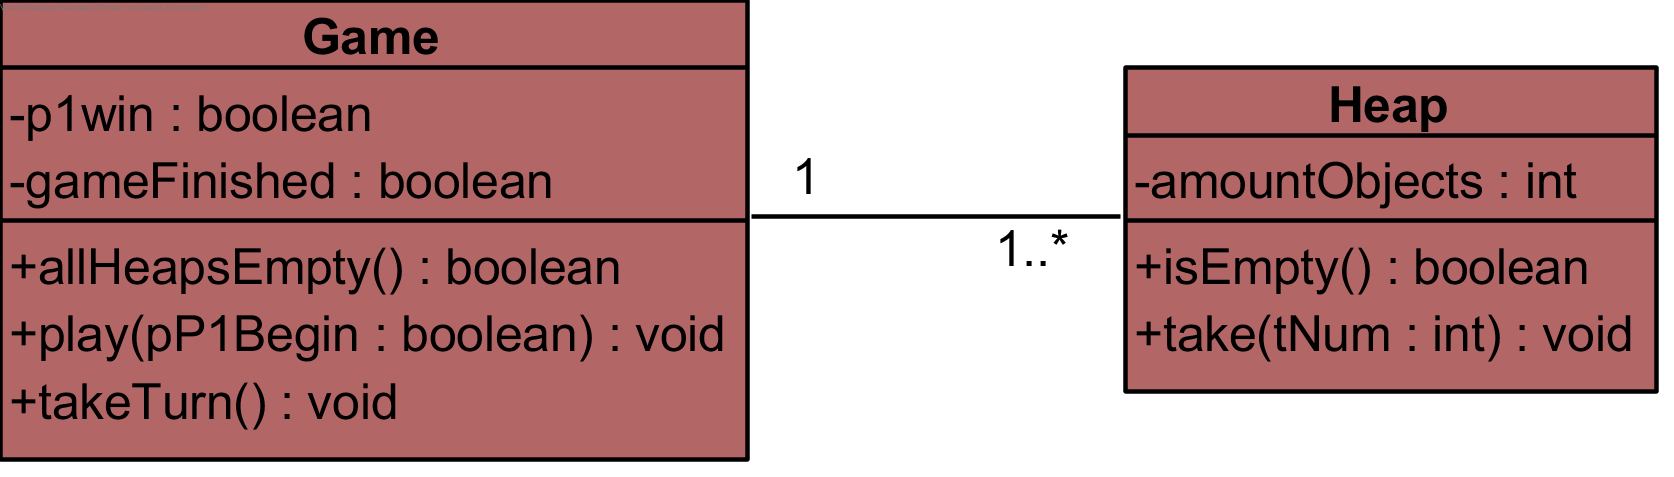
\includegraphics[width=0.75\textwidth]{chap-evaluatie/ClassDiagram1.png}
	\caption{Klassediagram voor Nim}
	\label{fig:nim-cd}
\end{figure}

De klasse \textit{Game} stelt het concept van een spel voor. \textit{p1Win} geeft aan of speler 1 heeft gewonnen en \textit{gameFinished} geeft aan of het spel volledig gespeeld is. \textit{allHeapsEmpty()} vraagt op of alle \textit{Heap}s leeg zijn. \textit{takeTurn()} doet een speler zijn beurt spelen. \textit{play(boolean)} is de methode die het verloop van het spel regelt.

De klasse \textit{Heap} stelt stapels van objecten voor. \textit{numObjects} is het aantal objecten dat een stapel bevat. \textit{isEmpty()} geeft aan of de stapel leeg is en \textit{take(int)} neemt een aantal objecten weg van een stapel.

Naast het klassediagram, dat de structuur van het spel modelleert, stellen we ook een aantal sequentiediagrammen op die het verloop van het spel regelen.

We tonen hier het centrale sequentiediagram. De anderen zijn beschikbaar in bijlage \ref{app:design-nim}.

\begin{figure}
	\centering
	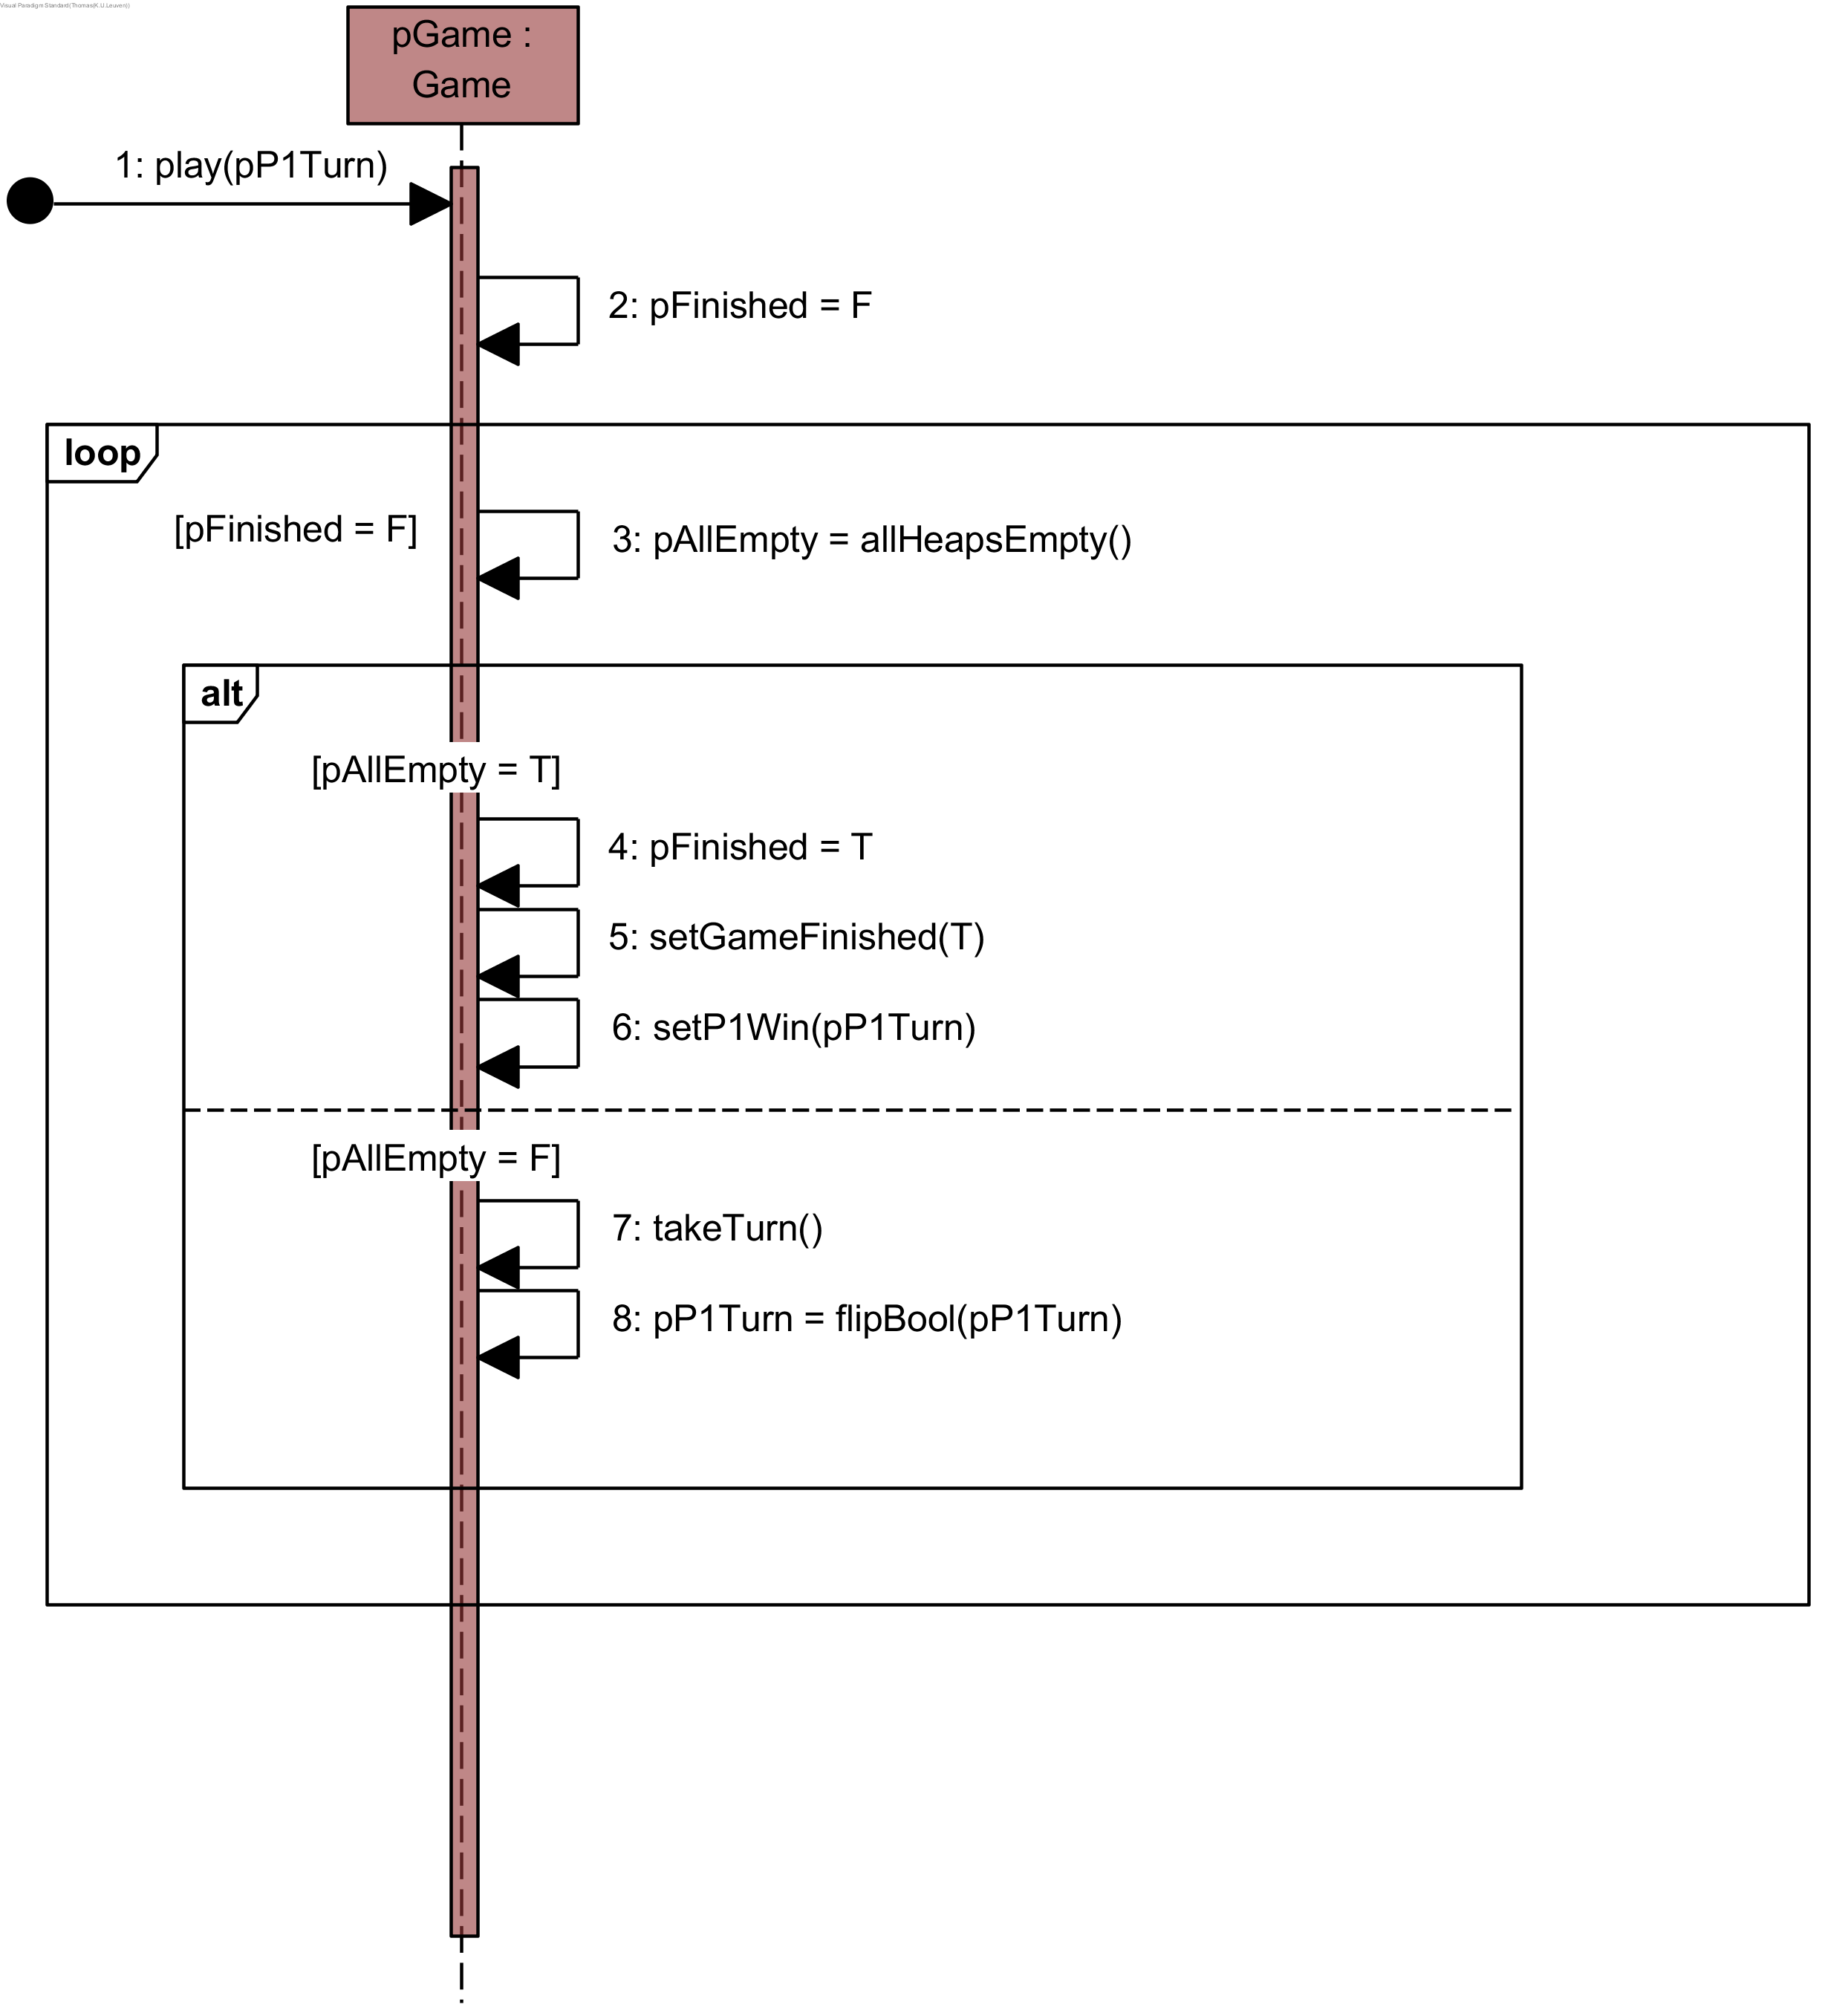
\includegraphics[width=0.8\textwidth]{chap-evaluatie/play.png}
	\caption{Sequentiediagram voor \textit{play(boolean)}}
	\label{fig:nim-play}
\end{figure}

Diagram \ref{fig:nim-play} bepaalt eerst of alle stapels leeg zijn. Zo ja, is het spel voorbij en is de speler die nu aan beurt is de winnaar. Zo nee, speelt de huidige speler een ronde en geeft de beurt door aan de andere speler.

Diagram \ref{fig:nim-allHeapsEmpty} vraagt aan alle stapels om de beurt of ze leeg zijn. Als het een stapel tegenkomt die niet leeg is, is het antwoord meteen nee. Als het enkel stapels tegenkomt die leeg zijn, is het antwoord ja.

Diagram \ref{fig:nim-isEmpty} antwoordt ja als de stapel leeg is en nee als de stapel niet leeg is.

Diagram \ref{fig:nim-takeTurn} vraagt aan de speler van welke stapel hij objecten wil nemen. Als de geselecteerde stapel leeg is, wordt er opnieuw gevraagd om een stapel te selecteren. Als de speler een stapel heeft gekozen die niet leeg is, moet hij kiezen om minstens \'e\'en en maximaal het aantal objecten dat nog overblijft op de stapel weg te nemen.

Diagram \ref{fig:nim-take} berekent hoeveel objecten er nog overblijven op een stapel gegeven een aantal objecten om weg te nemen van de stapel. Als het verschil kleiner is dan nul, wordt de teller op nul gezet.

Het IDP-bestand met de automatisch gegenereerde uitvoertheorie voor deze diagrammen is beschikbaar op de volgende online locatie: \url{https://pastebin.com/f90riJGV}.

%\begin{landscape}
%	\newpage
%	\thispagestyle{plain}
%	\begin{figure}-
%		\centering
%		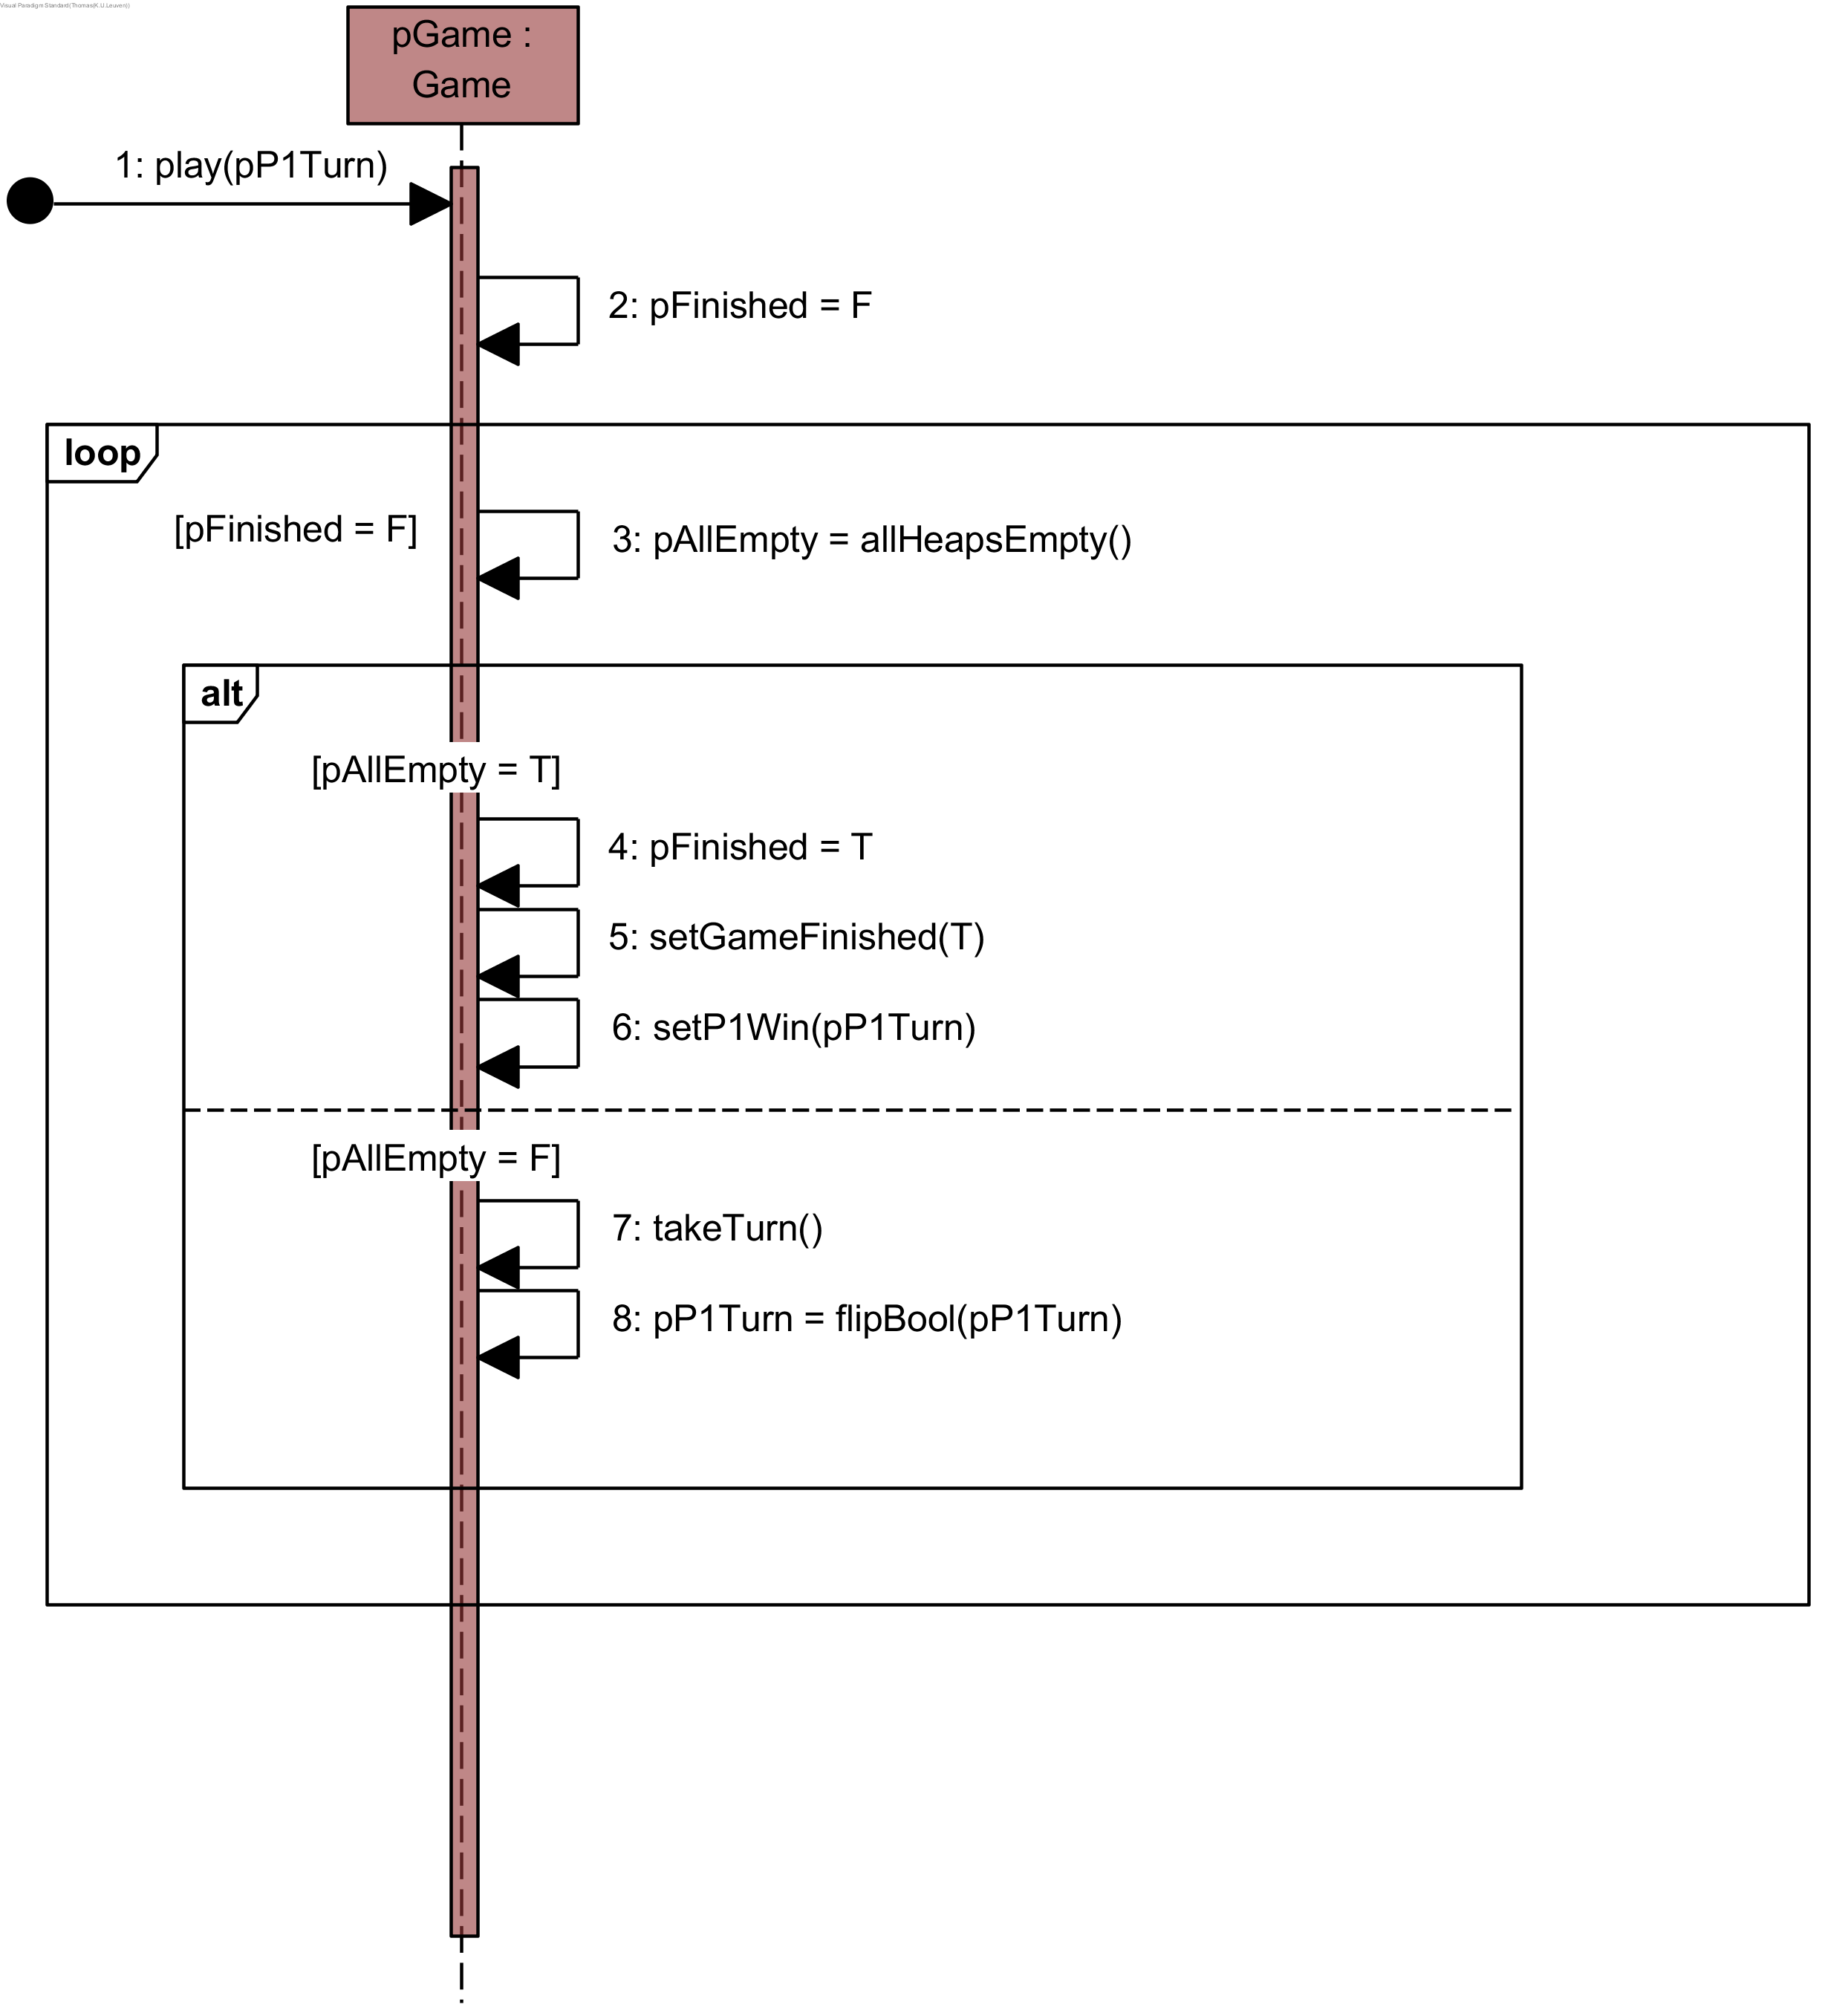
\includegraphics[width=0.4\textwidth]{chap-evaluatie/play.png}
%		\caption{Sequentiediagram voor play()}
%		\label{fig:nim-play}
%	\end{figure}
%	\begin{figure}
%		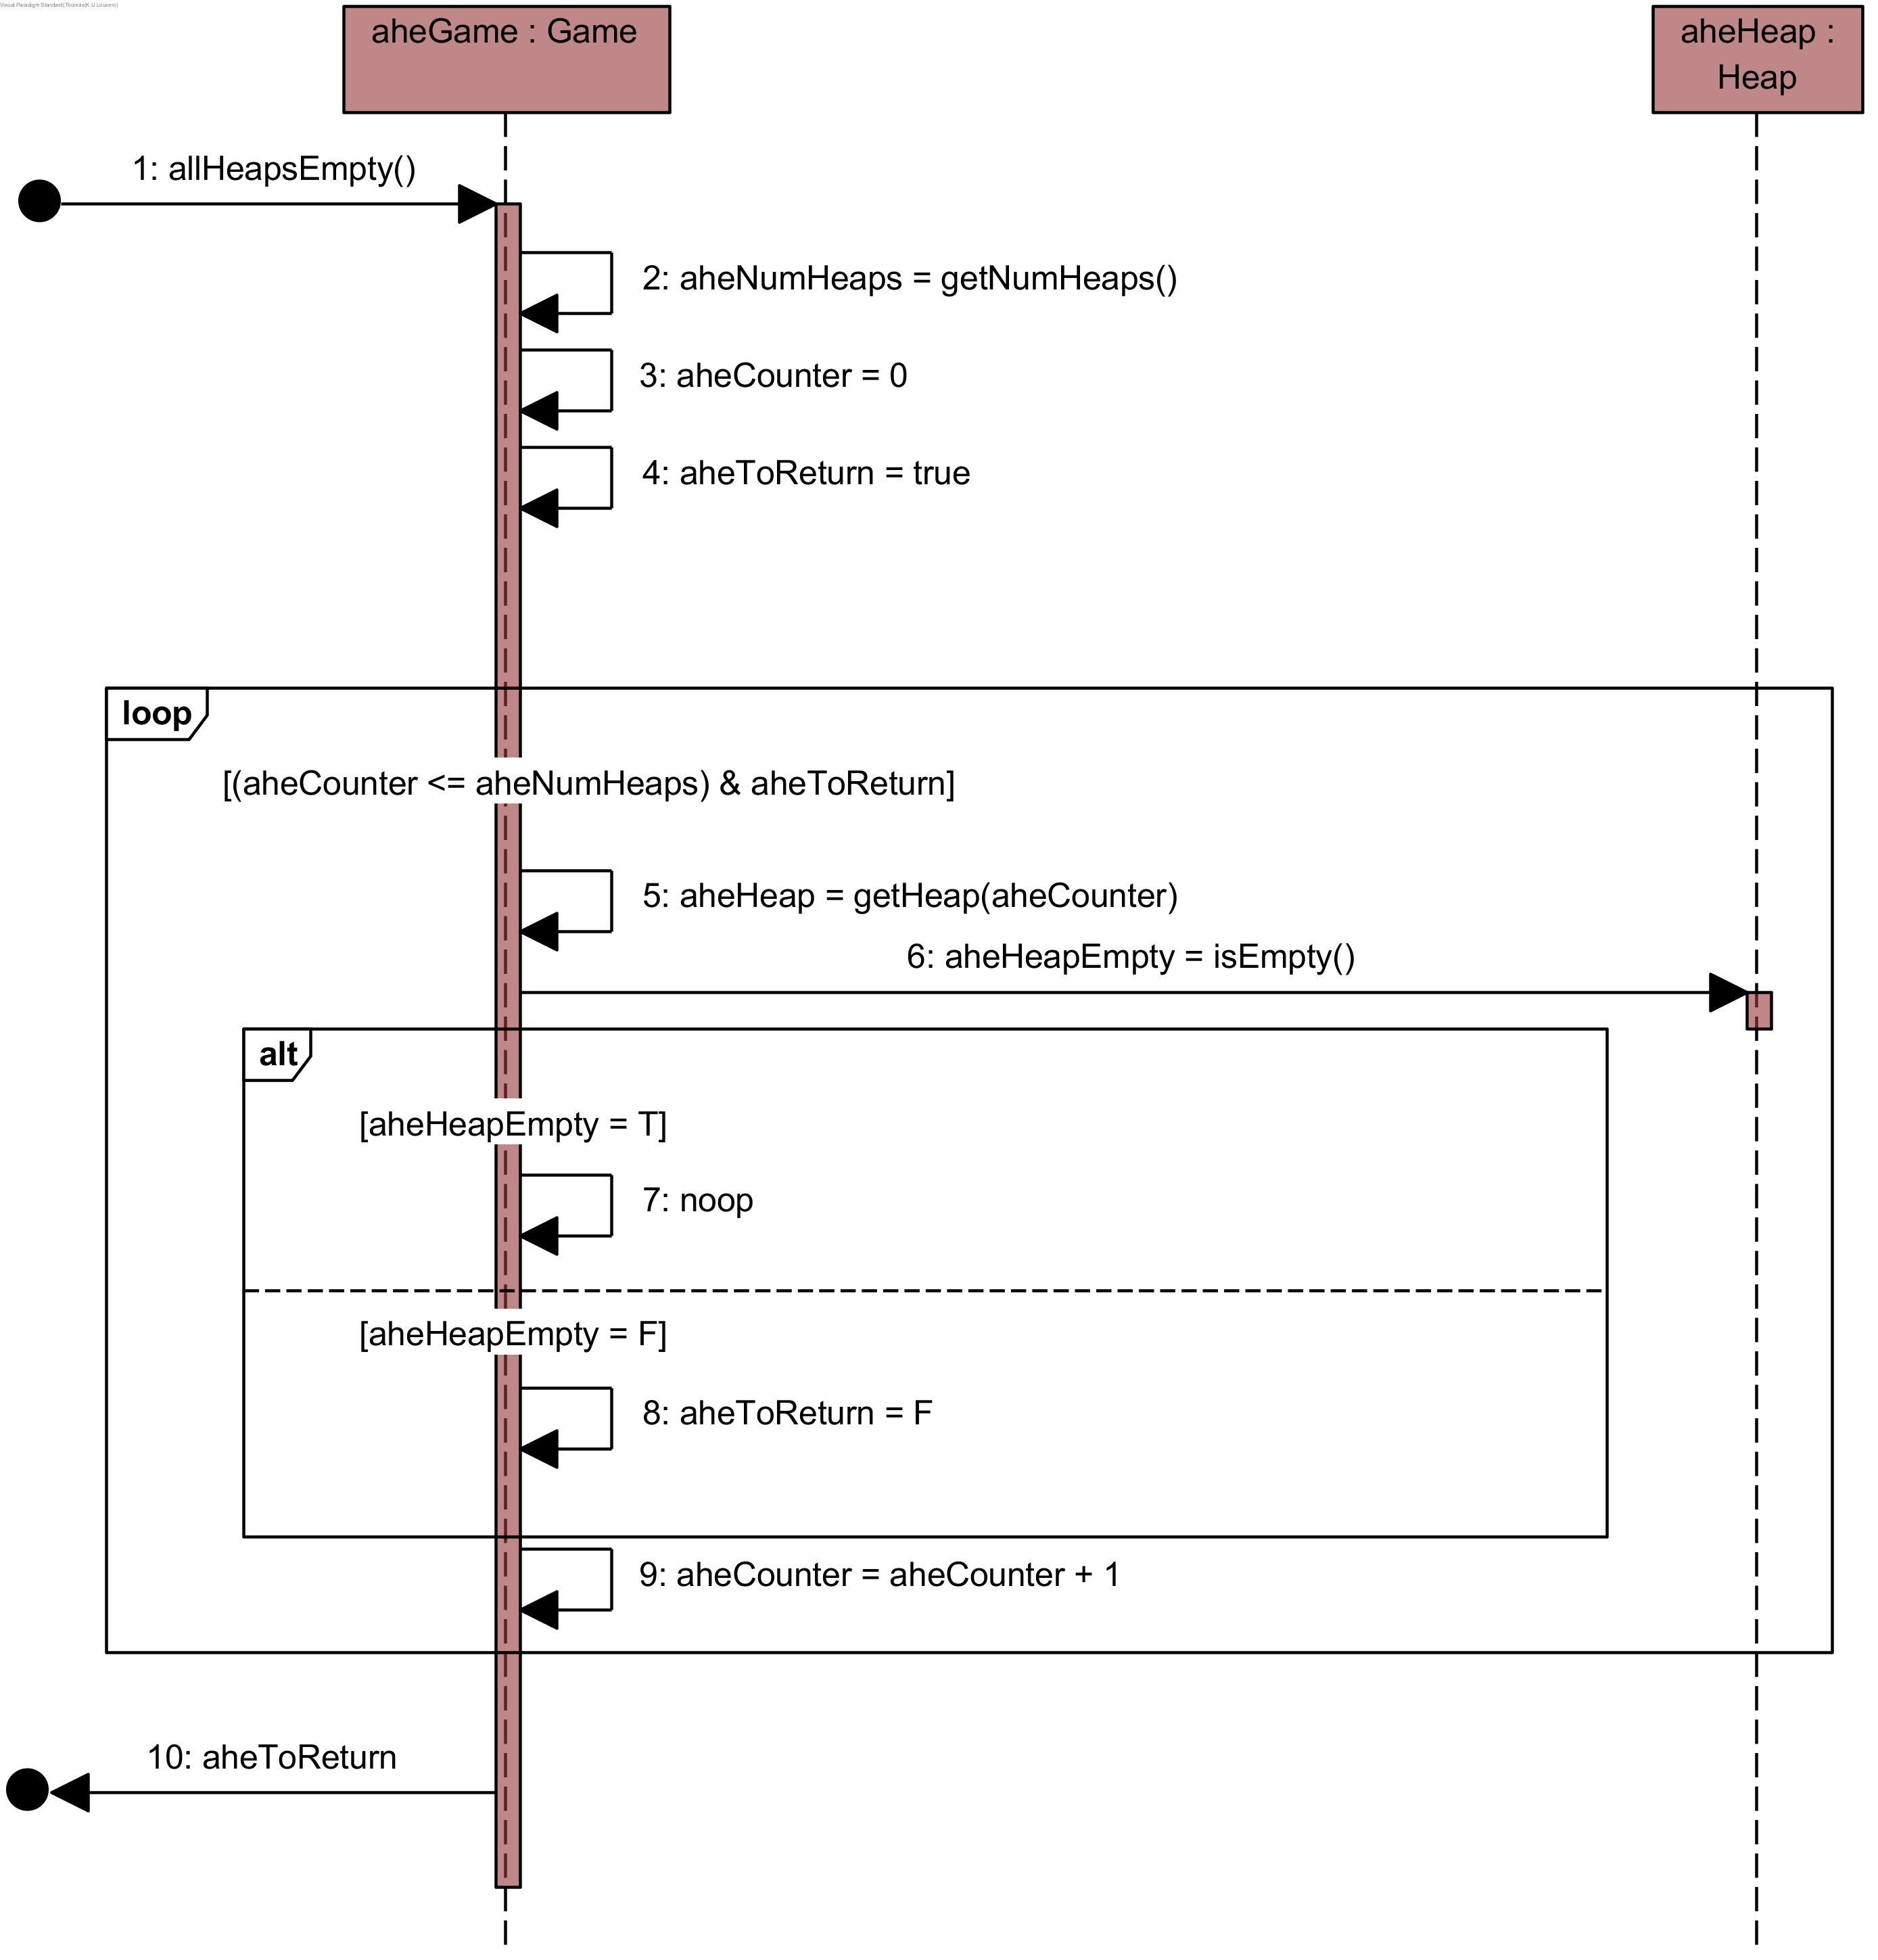
\includegraphics[width=0.75\textwidth]{chap-evaluatie/allHeapsEmpty.png}
%		\caption{Sequentiediagram voor allHeapsEmpty()}
%		\label{fig:nim-allHeapsEMpty}
%	\end{figure}
%\end{landscape}

\subsection{Ontwerp voor Reversi}\label{sec:reversi-design}

Reversi is een spel voor twee spelers. Ze spelen op een rechthoekig bord verdeeld in even grote vakken. Er liggen al in het begin stenen op het bord. De spelers leggen om de beurt een steen van hun kleur op het bord. Een steen mag enkel gelegd worden indien minstens \'e\'en steen van de tegenspeler ligt tussen de nieuwe steen en een steen van de eigen kleur die al op het bord ligt. Noem alle zulke stenen van de tegenspeler de gepakte stenen. Na het neerleggen van de nieuwe steen draait de speler de gepakte stenen om naar zijn kleur. Als geen enkele zet leidt tot minstens \'e\'en gepakte steen, slaat de speler zijn beurt over. Als de beurt twee keer na elkaar wordt overgeslagen, stopt het spel. De speler met het grootste aantal stenen van zijn kleur wint.

Figuur \ref{fig:reversi-cd} bevat het klassediagram. Het toont twee klasses: \textit{Board} en \textit{Position}. \textit{Board} houdt bij wat de grootst mogelijke x- en y-co\"ordinaten zijn, of het spel voorbij is, of zwart de winnaar is en of het gelijkspel is. \textit{Position} houdt bij wat de co\"ordinaten zijn, of het vak bezet is en of er een zwarte steen op ligt.

\begin{figure}
	\centering
	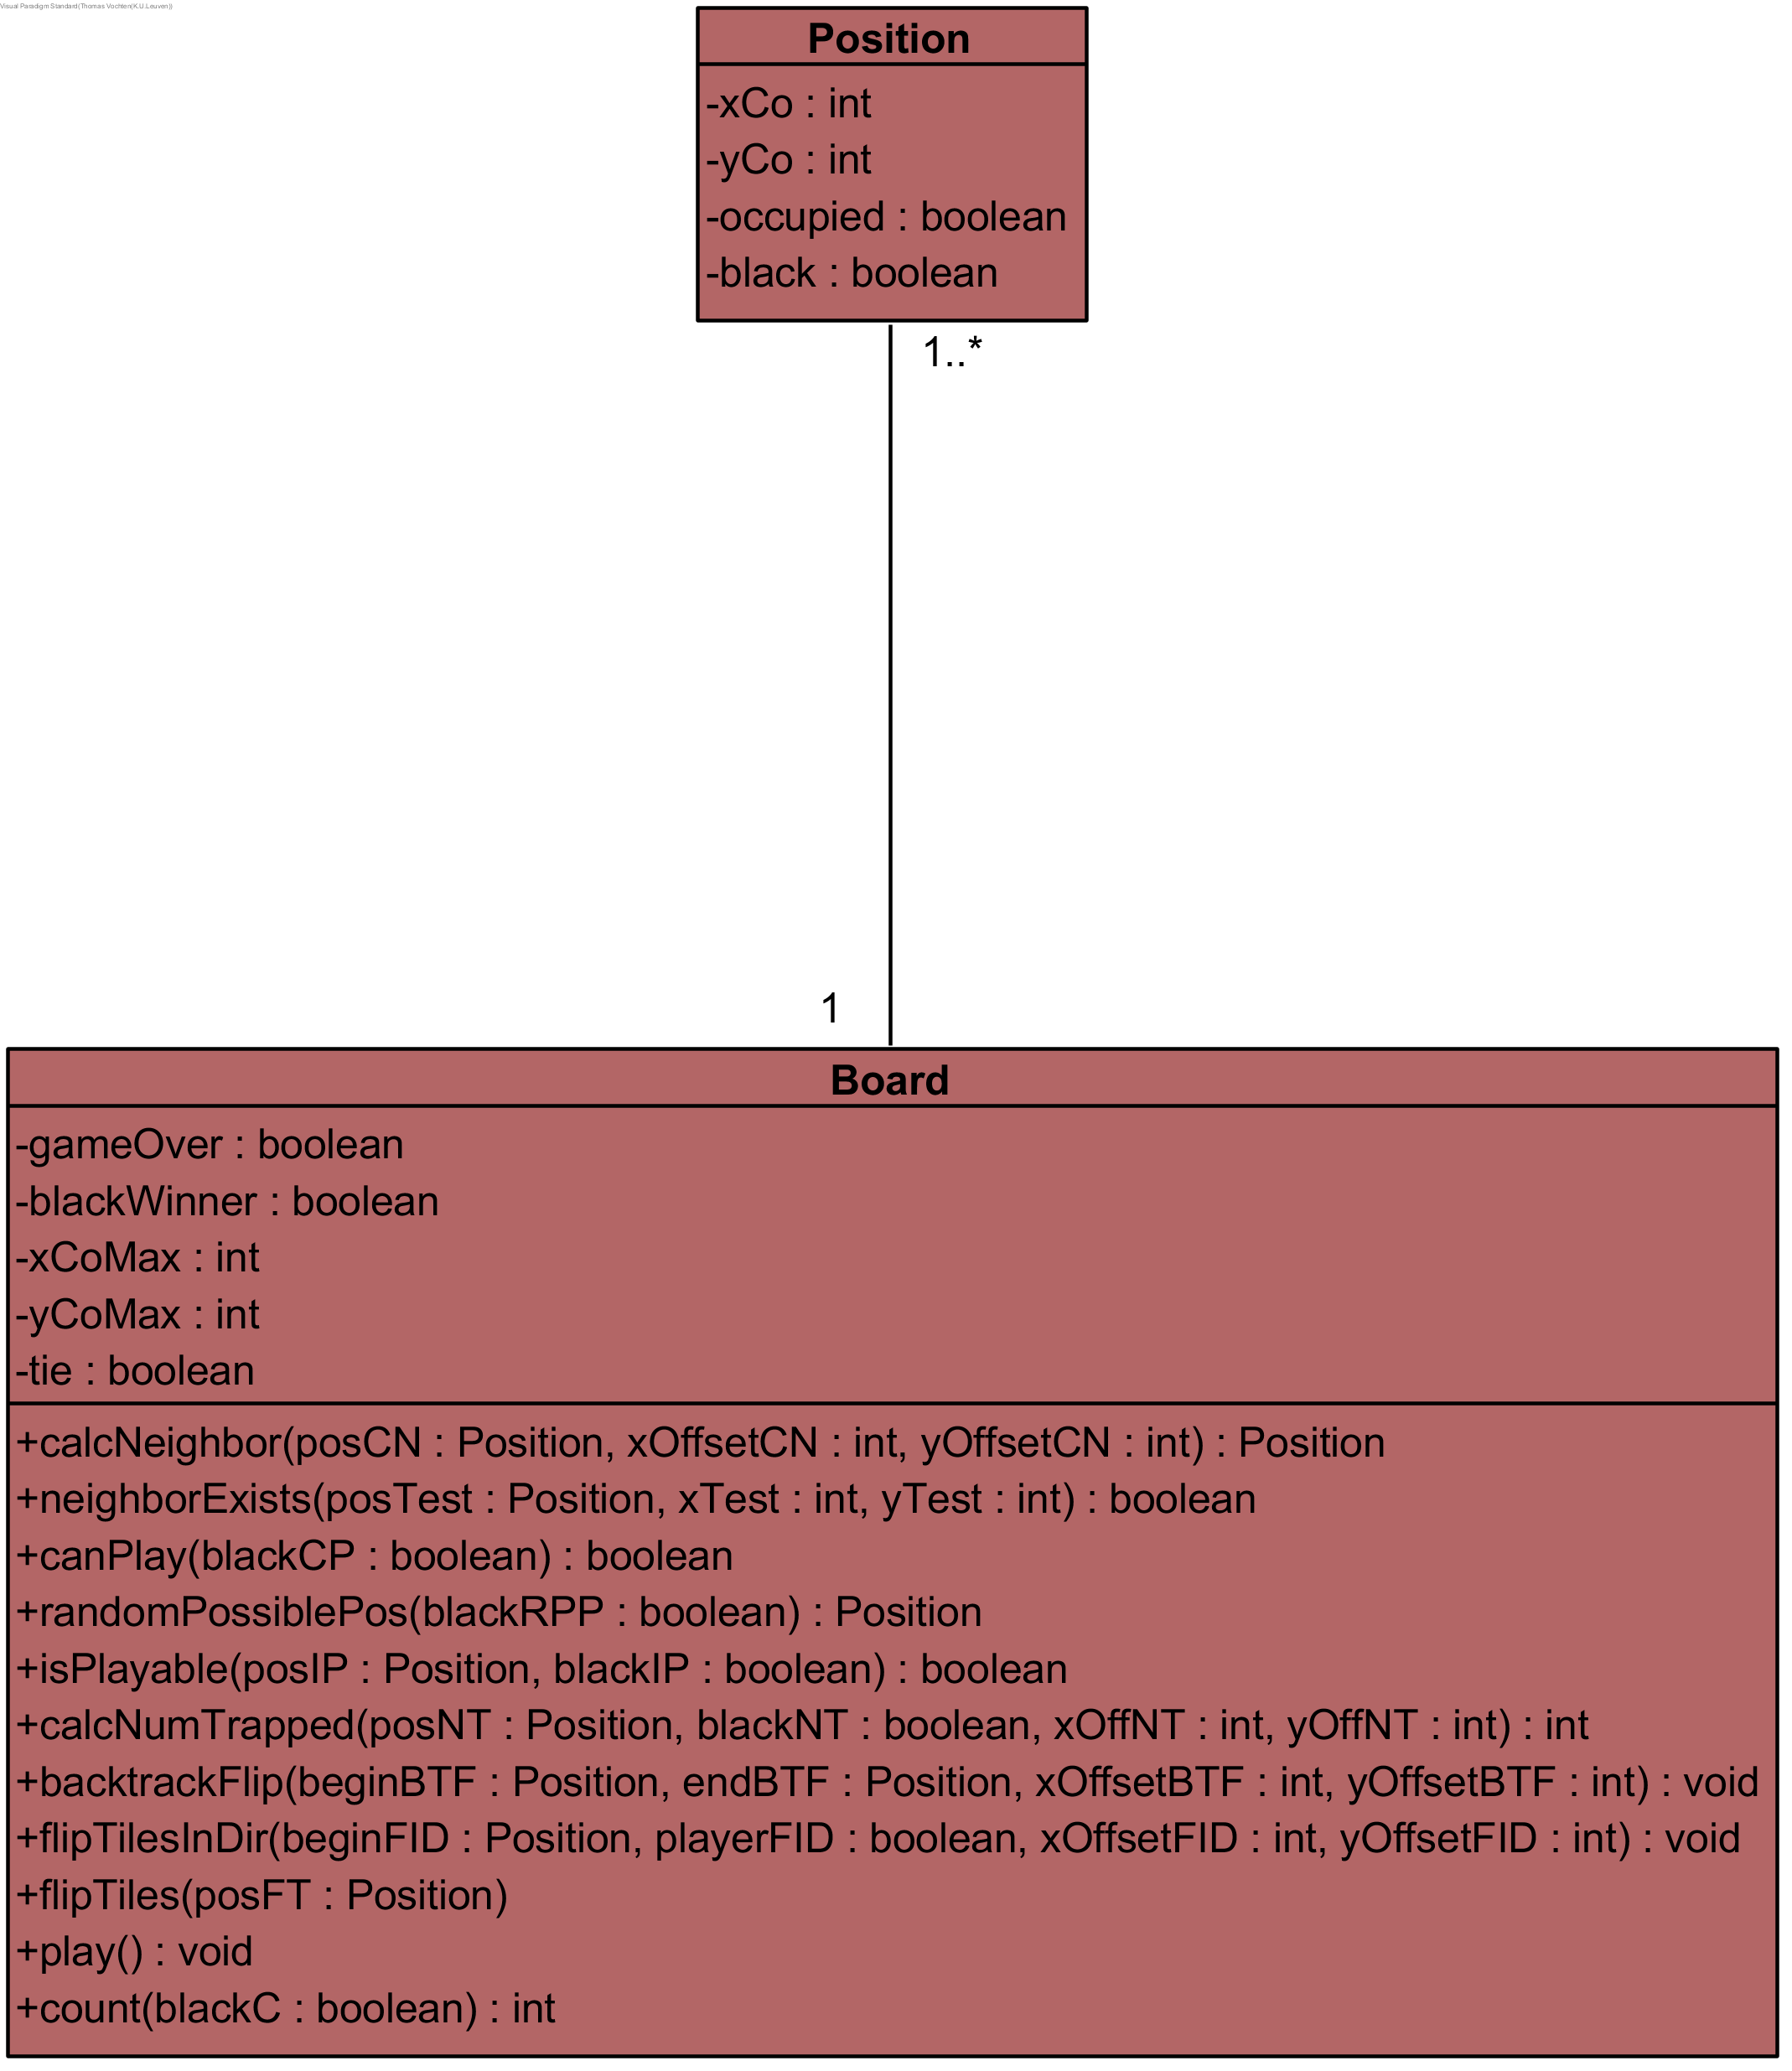
\includegraphics[width=0.7\textwidth]{chap-evaluatie/reversi-cd.png}
	\caption{Het klassediagram voor Reversi}
	\label{fig:reversi-cd}
\end{figure}

De sequentiediagrammen zijn beschikbaar op deze locatie: \url{https://imgur.com/a/kgVg4dv} 

\textit{play()} regelt het spelverloop. Aan het begin van elke beurt wordt er gecontroleerd of de huidige speler een zet kan doen. Zo ja, kiest de speler een positie en legt er een steen. Zo nee slaat de speler zijn beurt over. Als de beurt twee keer wordt overgeslagen, wordt voor beide spelers het aantal stenen geteld en wordt de winnaar aangeduid, tenzij het gelijkspel is.

\textit{canPlay(boolean)} controleert voor elk vak om de beurt of de gegeven speler een steen op dat vak kan leggen. Het antwoordt ja zodra het een geldig vak vindt. Als geen enkel vak geldig is, antwoordt het nee.

\textit{isPlayable(Position, boolean)} gaat voor de gegeven positie na of het een geldige zet zou zijn om daar een steen te leggen. De methode controleert voor elke richting om de beurt of minstens \'e\'en steen van de tegenspeler omgedraaid zou worden. Het antwoord is ja als en slechts als zulk een richting bestaat. 

\textit{calcNumTrapped(Position, boolean, int, int)} berekent voor de gegeven positie, speler en richting hoeveel stenen hij zou pakken als hij daar een steen legde. Het houdt een teller bij van het aantal gepakte stenen. De methode bekijkt telkens de buurpositie in de gegeven richting. Als er een steen van de tegenspeler ligt, wordt de teller verhoogd met \'e\'en. Als er geen steen ligt, wordt de teller op nul gezet en stopt de uitvoering van de lus. Als er een steen ligt van de eigen kleur, is het correcte aantal gepakte stenen berekend en stopt de uitvoering van de lus ook. Het antwoord is de uiteindelijke waarde van de teller.

\textit{neighborExists(Position, int, int)} controleert of er voor de gegeven positie in de gegeven richting een buur bestaat. Het antwoord is ja als en slechts als de resulterende x- of y-co\"ordinaat ligt tussen nul en de grootst mogelijke co\"ordinaat.

\textit{calcNeighbor(Position, int, int)} haalt voor de gegeven positie en richting de buur op.

\textit{choosePossiblePos(boolean)} vraagt aan de gegeven speler om een x- en y-co\"ordinaat in te geven. De methode geeft de resulterende positie als antwoord als die positie speelbaar is. De uitvoering van de methode stopt niet tot de speler een geldige positie kiest.

\textit{flipTiles(Position)} draait voor de gegeven positie de stenen in alle mogelijke richtingen.

\textit{flipTilesInDir(Position, boolean, int, int)} beheerst het proces waarbij stenen gedraaid worden. De bedoeling is dat er in de gegeven richting de positie wordt gevonden van waaruit er stenen gedraaid kunnen worden. Daarom bekijkt de methode eerst de onmiddelijke buur. Als daar geen steen van de tegenspeler ligt, stopt de methode meteen. Daarna bekijkt de methode om de beurt een nieuwe buur. Als daar een steen van de tegenspeler ligt, gaat de lus verder. Als er geen steen ligt, stopt de methode. Als er een steen van de eigen kleur ligt, wordt er begonnen met het draaien van stenen vanaf die positie.

\textit{backtrackFlip(Position, Position, int, int)} draait in de gegeven richting alle stenen tot het gegeven stoppunt bereikt is.

\textit{count(boolean)} telt voor de gegeven speler hoeveel stenen er liggen van zijn kleur. Hierbij worden alle x- en y-co\"ordinaten bekeken.

Het IDP-bestand met de automatisch gegenereerde uitvoertheorie voor deze diagrammen is beschikbaar op de volgende online locatie: \url{https://pastebin.com/B1zKWyTq}.

\subsection{Evaluatie van het ontwerpproces}

Deze sectie evalueert criterium \ref{crit:design}.

\subsubsection{Evaluatie van het ontwerpproces voor Nim}

Door de beperkingen opgesomd in sectie \ref{sec:beperkingen} zijn er een aantal onintu\"itieve elementen. Als het mogelijk was geweest om de associaties van een object aan te passen tijdens de uitvoering, zou er een klasse \textit{Player} zijn geweest en een associatie \textit{Game}---\textit{Player} die de winnaar aanduidt. Aangezien er maar twee spelers zijn, is het echter voldoende om de winnaar voor te stellen met een booleaanse waarde. Als \textit{gameFinished} waar is, kan toch de winnaar ondubbelzinnig aangeduid worden.

Nim is een simpel spel, dus waren er geen noemenswaardige moeilijkheden bij het ontwerp van de diagrammen. Omdat men maar relatief simpele taken kan doen met \'e\'en enkele instructie, leidt dit er wel toe dat er een veelvoud aan instructies nodig zijn, wat de tijd die nodig is om het ontwerp te maken verhoogt.

\subsubsection{Evaluatie van het ontwerpproces voor Reversi}

Ook hier leiden de beperkingen opgesomd in sectie \ref{sec:beperkingen} tot een groot aantal instructies. In dit ontwerp ontbreekt er ook een klasse \textit{Player} omdat de associaties van een object niet aangepast kunnen worden tijdens de uitvoering. \textit{Player} zou gebruikt kunnen worden om de winnaar aan te duiden en om voor een bepaalde \textit{Position} bij te houden of er een steen van die speler ligt.

Het zou in \textit{choosePossiblePos(boolean)} gebruiksvriendelijker zijn om eerst een lijst van mogelijke posities te berekenen en dan de speler de keuze te bieden in die lijst. Dit kan echter niet omdat variabelen geen verzameling kunnen voorstellen.

De diagrammen die voor een positie bepalen of er een steen gelegd kan worden en de diagrammen die het draaien van stenen verzorgen stellen eenvoudige algoritmes voor. Er waren echter relatief veel instructies nodig om ze te modelleren. Dit leidde ertoe dat het opstellen van deze diagrammen enkele uren duurde.

\subsection{Conclusie}\label{sec:design-conclusion}

Het is mogelijk om Nim en Reversi te modelleren in sequentiediagrammen en deze diagrammen te vertalen naar FO($\cdot$). Sequentiediagrammen zijn bedoeld voor een imperatieve stijl van programmeertalen. Dit leidt ertoe dat er een veelvoud aan instructies en variabelen nodig zijn om niet-triviale taken uit te voeren. Deze variabelen worden allemaal inertieel gemaakt, wat zorgt voor drie zinnen per variabele in de uitvoertheorie. Het gevolg hiervan is dat de resulterende IDP-bestanden omvangrijke vocabularia en theorie\"en bevatten. De grootte van de theorie stijgt verder omwille van de volgende zaken:

\begin{itemize}
	\item E\'en zin per diagram als minstens \'e\'en ander diagram het oproept.
	\item Zoveel zinnen als er parameters zijn voor een diagram bij elke oproep om een waarde toe te kennen aan elke parameter.
	\item E\'en zin per oproep van een diagram om het terugkeerpunt te zetten.
	\item E\'en of meerdere zinnen per gecombineerd fragment om de uitvoering ervan in goede banen te leiden.
\end{itemize}

\section{Simulatie van de spellen met de uitvoertheorie\"en}

Deze sectie evalueert criterium \ref{crit:simulation}.

Alle testen worden uitgevoerd op een machine die Ubuntu 16.04.3 LTS draait. Deze machine heeft als CPU de Intel(R) Core(TM)2 CPU 6600 en heeft 3969 MB aan geheugen beschikbaar. We gebruiken versie 3.7.0 van IDP.

We gebruiken de optie \textit{stdoptions.verbosity.groundingstats} om IDP te laten rapporteren over de rekentijd en het geheugengebruik in termen van de grootte van de \textit{grounding}\cite{DeCatBroes2014PLaa}. Daarnaast geven we ook het virtueel geheugengebruik.

IDP geeft voor progressie\"inferentie geen gegevens over de \textit{grounding}-grootte. Daarom rapporteren we in deze sectie enkel het virtueel geheugengebruik.

\subsection{Evaluatie van simulatie van Nim}

We spelen een spel met twee stapels. E\'en stapel bevat twee objecten en de andere bevat drie objecten.

De eerste speler neemt tijdens zijn beurt alle drie de objecten van de stapel met drie objecten. Vervolgens neemt de tweede speler \'e\'en object van de andere stapel. Nu heeft de eerste speler geen keuze en moet hij het overblijvend object nemen, waardoor hij het spel verliest.

Figuur \ref{fig:ms} bevat een boxplot van de rekentijd per simulatiestap, en figuur \ref{fig:ms-nooutliers} bevat een boxplot van dezelfde gegevens zonder de uitschieters. We zien dat voor ongeveer de helft van de tijdstappen de rekentijd tussen ongeveer 6,65 seconden en 6,9 seconden ligt. Globaal gezien is de rekentijd gespreid tussen ongeveer 6,5 seconden en 7,15 seconden. Omdat een procedurale modellering een groot aantal stappen tot gevolg heeft, duurt het ongeveer negentien minuten om het spel volledig te spelen. Van de 116 tijdstappen waren er vijf stappen waar de gebruiker het proces kon be\"invloeden, namelijk stappen 23, 34, 67, 78 en 111. De rekentijd tussen deze vijf stappen komt overeen met de verwachting die voortkomt uit de gemiddelde rekentijd.

\begin{figure}
	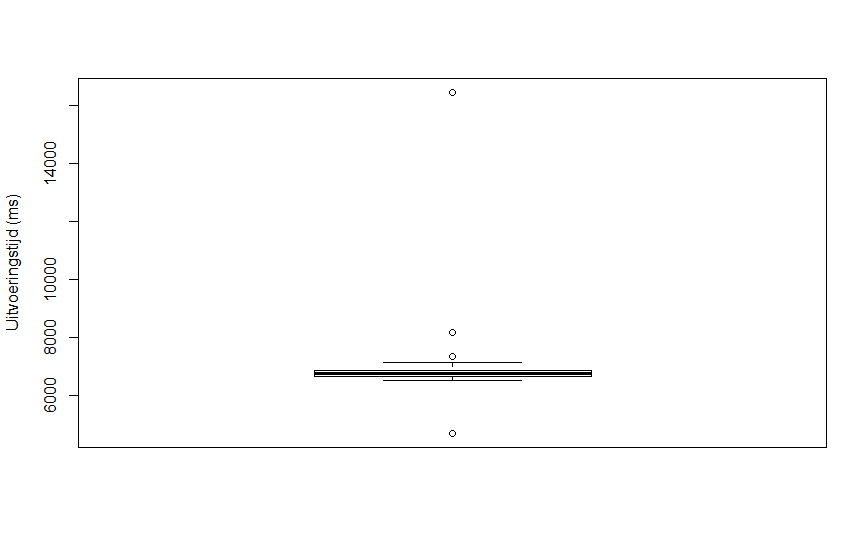
\includegraphics[width=1.05\textwidth]{chap-evaluatie/boxplot.png}
	\caption{Boxplot van de rekentijd per stap voor Nim}
	\label{fig:ms}
\end{figure}

\begin{figure}
	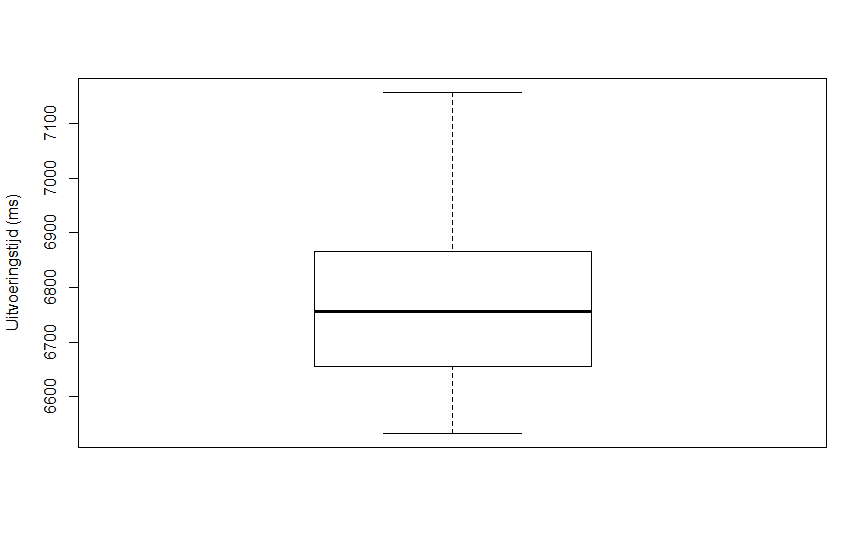
\includegraphics[width=1.05\textwidth]{chap-evaluatie/boxplotnooutliers.png}
	\caption{Boxplot van de rekentijd per stap zonder uitschieters voor Nim}
	\label{fig:ms-nooutliers}
\end{figure}

Tabel \ref{tab:sim-mem} bevat een overzicht van het virtueel geheugengebruik gemeten aan het begin van elke beurt.


\begin{table}[]
	\centering
	\begin{tabular}{|l|l|l|l|l|}
		\hline
		Beurt 1 & 0,91 GB  \\ \hline
		Beurt 2 & 2,09 GB  \\ \hline
		Beurt 3 & 3,34 GB  \\ \hline
		Einde   & 4,84 GB  \\ \hline
	\end{tabular}
	\caption{Virtueel geheugengebruik aan het begin van elke beurt voor Nim}
	\label{tab:sim-mem}
\end{table}

Uit deze resultaten blijkt dat we met de uitvoertheorie het spel kunnen spelen, maar het tijdsinterval tussen beurten is groot, en na enkele beurten wordt er al meerdere gigabytes aan virtueel geheugen gebruikt.

\subsection{Evaluatie van simulatie van Reversi}

We spelen een spel met de opstelling in figuur \ref{fig:reversigrid}.

De simulatie bereikt de vierde instructie van \textit{canPlay(boolean)}, maar daarna sluit IDP af vanwege een segmentatiefout. Het voerde dus in totaal acht stappen uit.

Figuur \ref{fig:reversi-time} geeft de rekentijd per stap weer. De grafiek heeft een lineair verloop. Het verschil tussen elke stap is ongeveer 300 seconden. Het duurt ongeveer 33 minuten om acht stappen uit te voeren. Dit suggereert dat het meerdere uren zou duren om een volledig spelverloop voor deze opstelling te simuleren.

Figuur \ref{fig:reversi-space} geeft het virtueel geheugengebruik per stap weer. Ook deze grafiek kent een lineair verloop. Het verschil tussen elke stap is ongeveer 125 megabyte. Om een volledig spelverloop voor deze opstelling te simuleren, zou er enkele tientallen aan gigabytes van geheugen nodig zijn.

\begin{figure}
	\centering
	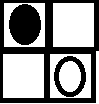
\includegraphics[width=0.15\textwidth]{chap-evaluatie/reversigrid.png}
	\caption{De opstelling voor de simulatie van Reversi}
	\label{fig:reversigrid}
\end{figure}

\begin{figure}
	\centering
	\begin{subfigure}{\textwidth}
		\centering
		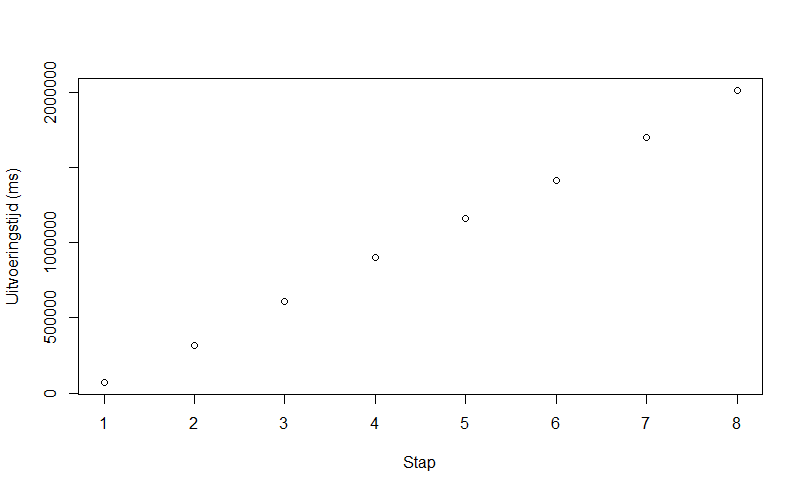
\includegraphics[width=\textwidth]{chap-evaluatie/reversi-time.png}
		\caption{Grafiek van de rekentijd per stap voor Reversi}
		\label{fig:reversi-time}
	\end{subfigure}
	\begin{subfigure}{\textwidth}
		\centering
		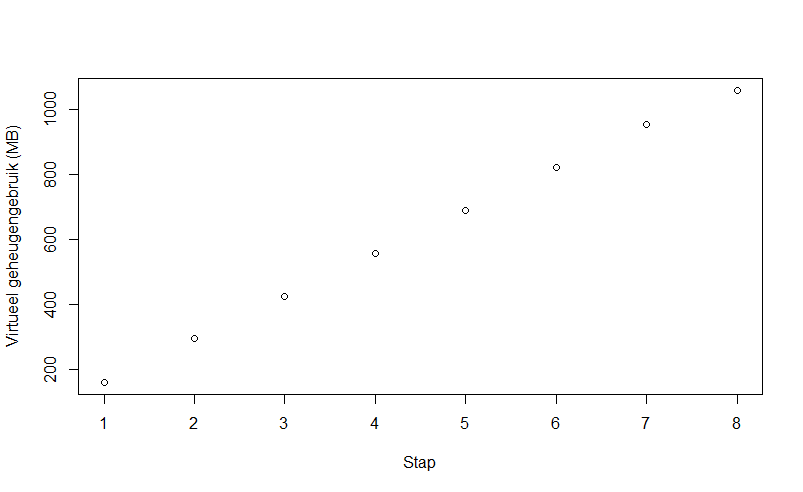
\includegraphics[width=\textwidth]{chap-evaluatie/reversi-space.png}
		\caption{Grafiek van het virtueel geheugengebruik per stap voor Reversi}
		\label{fig:reversi-space}
	\end{subfigure}
	\caption{Grafieken van de rekentijd en het virtueel geheugengebruik per stap voor Reversi}
	\label{fig:reversi-time-space}
\end{figure}

\subsection{Conclusie}

Het is mogelijk om Nim te spelen met de uitvoertheorie, maar dit kost ongeveer negentien minuten aan rekentijd en meerdere gigabytes aan geheugen voor een spel met twee stapels.

Het was mogelijk om acht stappen van progressie\"inferentie uit te voeren voor Reversi. Dit duurde echter 33 minuten en kostte een gigabyte aan geheugen.

Deze resultaten zijn te verklaren door:

\begin{itemize}
	\item Het groot aantal ternaire predicaten voor de variabelen gedefinieerd in de sequentiediagrammen.
	\item Het groot aantal \textit{SDPoint}s door omvangrijke diagrammen. Dit vergroot de zoekruimte voor \textit{SDPointAt/2} en \textit{ReturnPoint/3}.
	\item Omvangrijke theorie\"en, zoals besproken in sectie \ref{sec:design-conclusion}.
\end{itemize}

\section{Verificatie van de uitvoer van een sequentiediagram}\label{sec:verify-output}

Deze sectie evalueert criterium \ref{crit:output}.

We controleren de correctheid van de uitvoer van een diagram als volgt. Eerst stellen we zinnen op die ofwel correcte uitvoer ofwel incorrecte uitvoer beschrijven. Daarna voeren we voor elke zin modelexpansie uit. Daarbij voegen we de zin toe aan de uitvoertheorie en controleren we of we het verwachte resultaat krijgen. We geven telkens een invoerstructuur op van een beperkte grootte, maar die wel genoeg variatie toelaat om de uitvoering van een diagram te testen voor alle mogelijke invoerargumenten binnen een bepaald domein. Hierbij steunen we op de \textit{small-scope} hypothese\cite{andoni2003evaluating}, die stelt dat een groot aantal aan bugs in een programma ontdekt kan worden door het te testen voor alle mogelijke invoerargumenten binnen een beperkt domein.

\subsection{Verificatie van de correctheid van \textit{isEmpty()}}

We willen controleren of het diagram in figuur \ref{fig:nim-isEmpty} een positief antwoord geeft als en slechts als de gegeven stapel leeg is. We werken met een invoerstructuur die stelt dat de uitvoering begint met de eerste instructie van \textit{isEmpty} en eindigt na de laatste instructie van hetzelfde diagram. De invoerstructuur specificeert dat er in totaal zeven tijdstappen zijn.

Om de correctheid te controleren stellen we vier zinnen op:

\begin{align}
	\nonumber&\exists{t}[Time]\exists{st}[StackLevel]\exists{h}[Heap]\exists[n][LimitedInt](SDPointAt(t, finished) \\ &\land IeToReturnT(t, st, F) \land HeapamountObjects(t, h, n) \land n \leq 0).\label{form:ie_fnonempty} \\
	\nonumber&\exists{t}[Time]\exists{st}[StackLevel]\exists{h}[Heap]\exists[n][LimitedInt](SDPointAt(t, finished) \\ &\land IeToReturnT(t, st, T) \land HeapamountObjects(t, h, n) \land n > 0).\label{form:ie_fempty} \\
	\nonumber&\exists{t}[Time]\exists{st}[StackLevel]\exists{h}[Heap]\exists[n][LimitedInt](SDPointAt(t, finished) \\ &\land IeToReturnT(t, st, T) \land HeapamountObjects(t, h, n) \land n \leq 0).\label{form:ie_cempty} \\
	\nonumber&\exists{t}[Time]\exists{st}[StackLevel]\exists{h}[Heap]\exists[n][LimitedInt](SDPointAt(t, finished) \\ &\land IeToReturnT(t, st, F) \land HeapamountObjects(t, h, n) \land n > 0).\label{form:ie_cnonempty}
\end{align}

Zin \ref{form:ie_fnonempty} schrijft voor dat het antwoord negatief is, maar dat de stapel nul of minder objecten heeft.

Zin \ref{form:ie_fempty} is gelijkaardig, maar controleert op een positief antwoord met een stapel met meer dan nul objecten.

Beide zinnen moeten leiden tot een onvervulbare theorie.

Zin \ref{form:ie_cempty} schrijft voor dat het antwoord positief is en dat de stapel nul of minder objecten heeft.

Zin \ref{form:ie_cnonempty} controleert op een negatief antwoord met een stapel met meer dan nul objecten.

Beide zinnen moeten leiden tot een vervulbare theorie.

We voeren IDP viermaal uit met de voorgaande zinnen om de beurt toegevoegd aan de invoertheorie. Voor de twee eerste zinnen krijgen we inderdaad als antwoord dat de theorie onvervulbaar is. Voor zin \ref{form:ie_cempty} krijgen we een uniek model dat overeenkomt met een lege stapel. Voor zin \ref{form:ie_cnonempty} krijgen we alle modellen met een stapel die niet leeg is.

Er is een gelijkaardig tijdsverloop, \textit{grounding}-grootte en virtueel geheugengebruik voor alle vier de uitvoeringen. Het duurt ongeveer 40 seconden, de \textit{grounding}-grootte is 578 306 en het virtueel geheugengebruik is 2,14 GB.

We merken op dat het relatief lang duurt om modelexpansie uit te voeren voor dit diagram. De \textit{grounding} en het virtueel geheugengebruik zijn ook omvangrijk.

\subsection{Verificatie van de correctheid van \textit{allHeapsEmpty()}}\label{sec:verify-ahe}

We willen controleren of de functie zoals gemodelleerd in diagram \ref{fig:nim-allHeapsEmpty} een positief antwoord geeft als alle stapels leeg zijn en een negatief antwoord als minstens \'e\'en stapel niet leeg is. We werken met een invoerstructuur die aangeeft dat de uitvoering begint met de eerste instructie van \textit{allHeapsEmpty} en eindigt na de laatste instructie van dat diagram. De invoerstructuur specificeert dat er in totaal 25 tijdstappen en twee stapels zijn. Elke stapel kan nul tot vijf objecten bevatten.

We stellen vier zinnen op:

\begin{align}
	\nonumber&\exists{t}[Time]\exists{st}[StackLevel](SDPointAt(t, finished) \land AheToReturnT(t, st, F) \\ &\land \lnot\exists{h}[Heap]\exists{n}[LimitedInt](HeapamountObjects(t, h, n) \land n > 0)).\label{form:ahe_fnonempty} \\
	\nonumber&\exists{t}[Time]\exists{st}[StackLevel]\exists{h}[Heap]\exists[n][LimitedInt](SDPointAt(t, finished) \\ &\land AheToReturnT(t, st, T) \land HeapamountObjects(t, h, n) \land n > 0).\label{form:ahe_fempty} \\
	\nonumber&\exists{t}[Time]\exists{st}[StackLevel](SDPointAt(t, finished) \land AheToReturnT(t, st, T) \\ &\land \forall{h}[Heap]\forall{n}[LimitedInt](HeapamountObjects(t, h, n) \Rightarrow n \leq 0)).\label{form:ahe_cempty} \\
	\nonumber&\exists{t}[Time]\exists{st}[StackLevel]\exists{h}[Heap]\exists[n][LimitedInt](SDPointAt(t, finished) \\ &\land AheToReturn(t, st, F) \land HeapamountObjects(t, h, n) \land n > 0).\label{form:ahe_cnonempty}
\end{align}

Zin \ref{form:ahe_fnonempty} stelt voor dat het antwoord negatief is, maar dat er geen stapel bestaat met meer dan nul objecten.

Zin \ref{form:ahe_fempty} stelt voor dat het antwoord positief is, maar dat er een stapel bestaat met meer dan nul objecten.

Deze twee zinnen moeten leiden tot de conclusie dat de theorie onvervulbaar is.

Zin \ref{form:ahe_cempty} stelt voor dat het antwoord positief is en dat alle stapels leeg zijn.

Zin \ref{form:ahe_cnonempty} stelt voor dat het antwoord negatief is en dat er een stapel bestaat met meer dan nul objecten.

De conclusie moet hier zijn dat de theorie vervulbaar is.

Wanneer we IDP viermaal uitvoeren met deze vier zinnen om de beurt toegevoegd aan de uitvoertheorie, is de theorie inderdaad onvervulbaar voor de eerste twee zinnen. Zin \ref{form:ahe_cempty} leidt tot een uniek model dat overeenkomt met het geval dat alle stapels leeg zijn. Zin \ref{form:ahe_cnonempty} geeft alle modellen waar minstens \'e\'en stapel meer dan nul objecten heeft.

De uitvoeringstijd en \textit{grounding}-grootte zijn gelijkaardig voor alle vier uitvoeringen. De uitvoering duurt ongeveer 43,29 seconden, de \textit{grounding}-grootte is 366 643 en het virtueel geheugengebruik is 1,63 GB.

\subsection{Verificatie van een incorrecte modelling van allHeapsEmpty()}

We vervangen de achtste instructie van diagram \ref{fig:nim-allHeapsEmpty} door \textit{aheToReturn = T}. Dit leidt er dus toe dat het antwoord \textit{true} is zelfs als er een niet-lege stapel is.

We voeren IDP uit met zin \ref{form:ahe_fempty} toegevoegd aan de resulterende uitvoertheorie. Daarbij gebruiken we dezelfde invoerstructuur als in \ref{sec:verify-ahe}. Modelexpansie geeft alle modellen waar minstens \'e\'en stapel niet leeg is, maar waar de uitvoer van het diagram toch \textit{true} is. Aangezien deze theorie bij een correcte modellering onvervulbaar moet zijn, is de conclusie dat het diagram incorrect is.

\subsection{Verificatie van de correctheid van \textit{calcNeighbor(Position, int, int)}}\label{sec:verify-neighbor}

We willen controleren of het diagram voor \textit{calcNeighbor(Position, int, int)} de juiste buur teruggeeft voor elke positie. We werken met een invoerstructuur die stelt dat er tien tijdstappen zijn en dat er twee posities bestaan die horizontaal naast elkaar liggen.

Dit zijn de gebruikte zinnen:

\begin{align}
	\nonumber&\forall{t}[Time]\forall{st}[StackLevel]\forall{pr}[Position]((NeighborCNT(t, st, pr) \\ \nonumber &\land SDPointAt(t, finished)) \Leftrightarrow \exists{pi}[Position]\exists{xr}[LimitedInt]\exists{yr}[LimitedInt]\\ \nonumber &\exists{xi}[LimitedInt]\exists{yi}[LimitedInt]\exists{xo}[LimitedInt]\exists{yo}[LimitedInt](PosCNT(t, st, pi) \\ \nonumber &\land PositionxCo(t, pi, xi) \land PositionyCo(t, pi, yi) \land PositionxCo(t, po, xo) \\ \nonumber &\land PositionyCo(t, po, yo) \land XOffCNT(t, st, xo) \land YOffCNT(t, st, yo) \\ &\land xr = xi + xo \land yr = yi + yo)).\label{form:correct-neighbor} \\
	\nonumber&\forall{t}[Time]\forall{st}[StackLevel]\forall{pr}[Position]((NeighborCNT(t, st, pr) \\ \nonumber &\land SDPointAt(t, finished)) \Rightarrow \exists{pi}[Position]\exists{xr}[LimitedInt]\exists{yr}[LimitedInt]\\ \nonumber &\exists{xi}[LimitedInt]\exists{yi}[LimitedInt]\exists{xo}[LimitedInt]\exists{yo}[LimitedInt](PosCNT(t, st, pi) \\ \nonumber &\land PositionxCo(t, pi, xi) \land PositionyCo(t, pi, yi) \land PositionxCo(t, po, xo) \\ \nonumber &\land PositionyCo(t, po, yo) \land XOffCNT(t, st, xo) \land YOffCNT(t, st, yo) \\ &\land \lnot{}(xr = xi + xo \land yr = yi + yo))).\label{form:incorrect-neighbor}
\end{align} 

Zin \ref{form:correct-neighbor} stelt dat het verschil voor de x- en y-co\"ordinaat tussen de resulterende positie en de invoerpositie gelijk moet zijn aan het verschil tussen de co\"ordinaat van de resulterende afstand en de gegeven sprong. Deze zin moet dus leiden tot modellen waar de juiste buur wordt berekend.

Zin \ref{form:incorrect-neighbor} stelt dat dat verschil niet mag gelden voor de resulterende positie. Met deze zin moet de theorie dus onvervulbaar zijn.

Wanneer we modelexpansie uitvoeren voor deze twee zinnen, kan IDP echter niet tot een antwoord komen voordat het geheugen uitgeput is. We kunnen dus niet verifi\"eren of de uitvoer van dit diagram correct is.

\subsection{Conclusie}

Het is mogelijk om voor diagrammen \ref{fig:nim-isEmpty} en \ref{fig:nim-allHeapsEmpty} te verifi\"eren dat de uitvoer correct is. Dit duurde telkens minder dan een minuut met een \textit{grounding}-grootte van enkele honderduizenden. Het virtueel geheugengebruik voor \textit{isEmpty()} was 2,14 GB en voor \textit{allHeapsEmpty()} 1,62 GB.

Het geheugen raakte uitgeput bij het verifi\"eren van de uitvoer van het diagram voor \textit{calcNeighbor(Position, int, int)}. De verificatie kon niet succesvol uitgevoerd worden.

\section{Controleren op gewenste eigenschappen van het systeem als geheel}

Deze sectie evalueert criterium \ref{crit:properties}. We controleren of na de uitvoering van het systeem vanaf een bepaald startpunt tot aan een bepaald stoppunt een gewenste eigenschap van het systeem als geheel bewaard blijft. Dit doen we door zinnen op te stellen die deze voorwaarde uitdrukken en dan modelexpansie uit te voeren op de theorie met die zinnen eraan toegevoegd. De invoerstructuur bepaalt dat de uitvoering begint met het startpunt. De zinnen die de eigenschap modelleren zorgen er dan voor dat de uitvoering stopt aan het stoppunt. Zoals in sectie \ref{sec:verify-output} maken we weer gebruik van de \textit{small-scope} hypothese. Deze suggereert dat de meeste fouten in een modellering gevonden kunnen worden met een invoerstructuur van een beperkte grootte. Als de nieuwe zinnen bij modelexpansie geen modellen uitsluiten die wel geldig zijn voor de theorie zonder de nieuwe zinnen, is er een grote zekerheid dat de gewenste eigenschap geldt in het ontwerp.

\subsection{Correct verloop van een beurt in Nim controleren}

Een beurt in Nim verloopt correct indien aan de volgende twee voorwaardes is voldaan:

\begin{itemize}
	\item Als minstens \'e\'en stapel niet leeg is, moet minstens \'e\'en stapel minder objecten bevatten aan het einde van de beurt dan aan het begin van de beurt.
	\item Als minstens \'e\'en stapel niet leeg is, mag ten hoogste \'e\'en stapel minder objecten bevatten aan het einde van de beurt dan aan het begin van de beurt.
\end{itemize}

Om dit te controleren, voegen we extra zinnen toe aan de gegenereerde theorie. We defini\"eren eerst twee hulppredicaten:

\begin{itemize}
	\item \textit{Empty(Time, Heap)}: De stapel is leeg op een bepaald tijdstip.
	\item \textit{LosesObject(Time, Heap)}: De stapel bevat aan het einde van de beurt minstens \'e\'en object minder.
\end{itemize}

Diagram \ref{fig:nim-takeTurn} modelleert het gedrag van een beurt. We willen controleren of een beurt voldoet aan de twee genoemde voorwaardes. Om deze controle eenvoudiger te maken, wordt verondersteld dat de uitvoering wordt beperkt tot \'e\'en uitvoering van \textit{takeTurn()}.
We voegen de volgende zinnen toe aan de theorie:

\begin{align}
	&\forall{t}[Time]\forall{h}[Heap](Empty(t, h) \Leftrightarrow HeapamountObjects(t, h, 0)).\label{form:heapempty} \\
	&\nonumber \forall{t}[Time]\forall{h}[Heap](LosesObject(t, h) \Leftrightarrow (SDPointAt(t, finished) \\ &\nonumber \land \exists{n_1}[LimitedInt]\exists{n_2}[LimitedInt](HeapamountObjects(Start, h, n_1) \\ &\land HeapamountObjects(t, h, n_2) \land n_2 < n_1))).\label{form:losesobject} \\
	&\nonumber \exists{h}[Heap](\lnot{}Empty(Start, h)) \Rightarrow \forall{t}[Time](SDPointAt(t, finished) \\ &\Rightarrow \exists!{h}[Heap](LosesObject(t, h)))\label{form:turncondition}.
\end{align}

Zin \ref{form:heapempty} stelt dat een stapel leeg is als het geen objecten bevat.

Zin \ref{form:losesobject} stelt dat alle stapels die strikt minder objecten bevatten aan het einde van de beurt dan aan het begin van de beurt lid moeten zijn van de interpretatie van \textit{LosesObject/2} wanneer de uitvoering het einde van het diagram heeft bereikt.

Zin \ref{form:turncondition} stelt dat als minstens \'e\'en stapel niet leeg is aan het begin van de beurt, dat exact \'e\'en stapel lid mag zijn van de interpretatie van \textit{LosesObject/2}.

We defini\"eren twee stapels in de invoerstructuur en zetten de initi\"ele \textit{SDPoint} naar de eerste instructie van \textit{takeTurn()}. Het duurt 24 tijdstappen om \textit{takeTurn()} volledig uit te voeren als meteen een niet-lege stapel wordt gekozen in instructie 3. Daarom defini\"eren we 24 tijdstappen. Een stapel kan tussen nul en twee objecten bevatten.

Modelexpansie geeft 40 modellen. Voor al de modellen waar \'e\'en van de twee stapels aan het begin minstens \'e\'en object heeft en de uitvoering het einde van het diagram bereikt, zien we inderdaad dat exact \'e\'en stapel minstens \'e\'en object verliest. Voor al de modellen waar beide stapels geen objecten bevatten, merken we dat de uitvoering het lusfragment nooit verlaat. IDP vindt ook alle modellen waar minstens \'e\'en stapel leeg is en waar die stapel telkens wordt gekozen. 

Voor 24 tijdstappen bereikt de uitvoering maximaal drie keer een instructie waar een stapel gekozen wordt en maximaal twee keer een instructie waar het aantal genomen objecten gekozen wordt. Samen met het feit dat er twee stapels zijn en dat ze tussen nul en twee objecten kunnen bevatten, leidt dit tot tabel \ref{tbl:exp-models} voor het aantal verwachte modellen per scenario

\begin{table}[]
	\centering
	\begin{tabular}{|l|l|l|}
\hline
Stapelgrootte & Aantal verwachte modellen & Som \\ \hline
0, 0          & 8                         & 8   \\ \hline
0, 1          & 4                         & 12  \\ \hline
0, 2          & 6                         & 18  \\ \hline
1, 0          & 4                         & 22  \\ \hline
1, 1          & 2                         & 24  \\ \hline
1, 2          & 3                         & 27  \\ \hline
2, 0          & 6                         & 33  \\ \hline
2, 1          & 3                         & 36  \\ \hline
2, 2          & 4                         & 40  \\ \hline
\end{tabular}
	\caption{Het aantal verwachte modellen per scenario}
	\label{tbl:exp-models}
\end{table}

Modelexpansie op de theorie waar zinnen \ref{form:heapempty}, \ref{form:losesobject} en \ref{form:turncondition} zijn aan toegevoegd vindt 40 modellen. De zinnen verminderen dus niet het aantal modellen dat wordt gevonden.

Het besluit is dat de toestand van het spel op een correcte manier verandert in de loop van \'e\'en beurt. Het toepassen van de \textit{small scope} hypothese leidt tot de conclusie dat het zeer waarschijnlijk is dat de toestand correct verandert over alle beurten heen voor alle mogelijke spelverlopen.

De \textit{grounding}-grootte voor deze uitvoering van modelexpansie is 1 596 587. De uitvoering duurt ongeveer 1 minuut en 16 seconden en het virtueel geheugengebruik is 5,19 GB.

\subsection{Correct verloop van een beurt in Reversi controleren}

Wanneer een speler een zet kan doen, is hij verplicht om dat te doen. We introduceren het hulppredicaat \textit{EmptyPos(Time, Position)}, wat aangeeft dat een bepaalde positie leeg is op een bepaald tijdstip.

We drukken de eigenschap uit voor de eerste speler. De volgende zinnen worden toegevoegd aan de theorie:

\begin{align}
	&\forall{t}[Time]\forall{p}[Position](EmptyPos(t, p) \Leftrightarrow Positionoccupied(t, p, F)).\label{form:emptypos} \\
	\nonumber &\forall{t}[Time](SDPointAt(t, play\_9post) \Rightarrow (\#\{p [Position] : EmptyPos(t, p)\} = \\ &\#\{p [Position] : EmptyPos(Start, p)\} - 1)).\label{form:onefewer}
\end{align}

De invoerstructuur specificeert een bord van twee rijen en twee kolommen. Het stelt ook dat de eerste instructie de vierde instructie van \textit{play()} is. Samen met het eindpunt genoemd in zin \ref{form:onefewer}, zorgt dit ervoor dat enkel scenario's waar de eerste speler een zet kan doen worden gecontroleerd. De theorie en structuur kunnen eenvoudig aangepast worden om te controleren voor de tweede speler.

Zoals in sectie \ref{sec:verify-neighbor}, kan IDP bij modelexpansie geen antwoord geven voordat het geheugen uitgeput raakt. Diezelfde sectie toont immers dat het geheugen uitgeput raakt bij het verifi\"eren van een diagram van negen instructies. Dit was dus te verwachten.

We kunnen deze eigenschap niet verifi\"eren voor dit ontwerp voor Reversi.

\subsection{Conclusie}

Voor Nim konden we nagaan dat een speler minstens \'e\'en object van exact \'e\'en stapel neemt als minstens \'e\'en stapel niet leeg is. Deze controle duurde langer dan een minuut, met een \textit{grounding}-grootte van ongeveer 1,6 miljoen en een virtueel geheugengebruik van 5,19 GB.

Het geheugen raakte uitgeput bij de controle of in ons ontwerp voor Reversi een speler exact \'e\'en steen op het bord legt indien het mogelijk is om een zet te doen.

\section{Samenvatting van de bevindingen}
We hebben ontwerpen voor Nim en Reversi gemaakt en ze kunnen vertalen naar FO($\cdot$)-theorie\"en. Dit was relatief eenvoudig, maar door de vele benodigde instructies duurde het relatief lang om de diagrammen te maken. Daarbij merkten we op dat een aantal factoren ervoor zorgen dat de resulterende vocabularia en theorie\"en een grote omvang aannemen.

We konden de uitvoertheorie voor Nim gebruiken om een spelverloop te simuleren. Dit duurde negentien minuten en kostte 4,84 GB aan geheugen. We konden Reversi maar deels simuleren omwege van een fout intern aan IDP. Daarbij kunnen we wel voorspellen dat het enkele uren zou duren om een beurt te spelen met een kost van enkele tientallen aan gigabytes aan geheugen.

Voor diagrammen \ref{fig:nim-isEmpty} en \ref{fig:nim-allHeapsEmpty} konden we verifi\"eren dat de uitvoer correct was. Modelexpansie duurde telkens minder dan een minuut, met een \textit{grounding}-grootte van enkele honderdduizenden en een maximaal virtueel geheugengebruik van 2,14 GB. We probeerden de uitvoer van \textit{calcNeighbor(Position, int, int)} te verifi\"eren, maar het geheugen raakte uitgeput voordat IDP een antwoord kon geven.

Voor het ontwerp voor Nim konden we nagaan dat als minstens \'e\'en stapel niet leeg is, dat de speler tijdens een beurt van exact \'e\'en stapel minstens \'e\'en object wegneemt. Deze controle duurde ongeveer 1 minuut en 16 seconden, met een \textit{grounding}-grootte van ongeveer 1,6 miljoen en een virtueel geheugengebruik van 5,19 GB. We probeerden na te gaan voor Reversi dat exact \'e\'en positie wordt ingenomen als een speler een zet kan doen. Ook hier raakte het geheugen echter uitgeput.

Zowel voor Nim als Reversi merken we dat de rekentijd en het geheugengebruik voor modelexpansie en progressie\"inferentie groot zijn. Het is dus interessant om te onderzoeken welke mogelijkheden er bestaan om sequentiediagrammen compacter te maken en zo ook de resulterende vocabularia en theorie\"en.